\documentclass[12pt]{article}
\usepackage{tikz}
\usepackage{amsmath}
% Underlining package
\usepackage{ulem}
\usetikzlibrary{calc}
\usepackage[a4paper, portrait, margin=1cm]{geometry}
\usepackage{fancyhdr}

\def \HeadingQuestions {\section*{\Large Name: \underline{\hspace{8cm}} \hfill Date: \underline{\hspace{3cm}}} \vspace{-3mm}
{Angles in Right Triangles: Questions} \vspace{1pt}\hrule}

% raise footer with page number; no header
\fancypagestyle{myfancypagestyle}{
  \fancyhf{}% clear all header and footer fields
  \renewcommand{\headrulewidth}{0pt} % no rule under header
  \fancyfoot[C] {\thepage} \setlength{\footskip}{14.5pt} % raise page number 6pt
}
\pagestyle{myfancypagestyle}  % apply myfancypagestyle

\newcounter{minipagecount}

\begin{document}
\HeadingQuestions
\vspace{8mm}

\begin{minipage}{0.55\textwidth}
  \refstepcounter{minipagecount}
  \noindent{(\theminipagecount)}\quad
  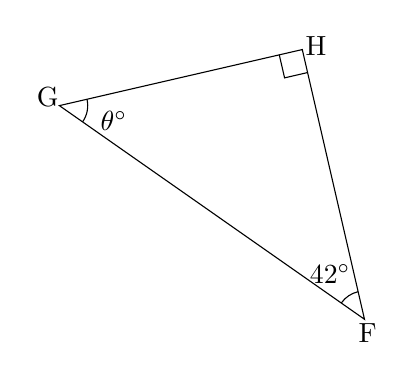
\begin{tikzpicture}[scale=1.2, baseline=(current bounding box.north)]

    \begin{scope}[rotate=325]
      \coordinate (A) at (0,0);
      \coordinate (B) at (3.941783758819614,0);
      \coordinate (C) at (intersection cs: first line={(A)--($(A)+(48:4cm)$)}, second line={(B)--($(B)+(180-42:4cm)$)});
      \draw (A) -- (B) -- (C) -- cycle;

      % Mark angles with arcs
      \draw ($(A)!0.3cm!(B)$) arc [start angle=0, end angle=48, radius=0.3cm];
      \draw ($(B)!0.3cm!(C)$) arc [start angle=180-42, end angle=180, radius=0.3cm];
      % \draw ($(C)!0.3cm!(A)$) arc [start angle=180+48, end angle=360-42, radius=0.3cm];
      % rt angle mark at C
      % \tkzMarkRightAng0le(A,C,B); % uses \usepackage{tkz-euclide}
      \draw ($(C)!0.25cm!(A)$) -- ($(C)!0.25cm!(A)!0.25cm!90:(A)$) -- ($(C)!0.25cm!(B)$);
      %  The ($(C)!0.3cm!(A)!0.3cm!90:(A)$) syntax is used to specify a point that is 0.3cm away from the point ($(C)!0.3cm!(A)$) in a direction that is perpendicular to the line connecting points C and A. This is achieved by first specifying the point ($(C)!0.3cm!(A)$) and then rotating it by 90 degrees around point A using the !angle:anchor syntax.

      % Label angles
      \node at ($(A)!-0.15cm!(B)$) {G};
      \node at ($(B)!-0.15cm!(C)$) {F};
      \node at ($(C)!-0.15cm!(A)$) {H};

      % Mark angles in degrees
      \coordinate (midBC) at ($(B)!0.5!(C)$);
      \node at ($(A)!0.60cm!(midBC)$) {$\theta^\circ$};

      \coordinate (midAC) at ($(A)!0.5!(C)$);
      \node at ($(B)!0.60cm!(midAC)$) {$42^\circ$};

      % \coordinate (midAB) at ($(A)!0.5!(B)$);
      % \node at ($(C)!0.55cm!(midAB)$) {<<angleCValueDisplay>>$^\circ$};

    \end{scope}
  \end{tikzpicture}
\end{minipage}%
\hfill
\begin{minipage}{0.4\textwidth}
  \begin{align*}
    \angle \text{G} &= 90^\circ - \angle \text{\dotuline{~~~~~~~}} \\
    &= 90^\circ - \dotuline{~~~~~~~}^\circ  \\
    &= \dotuline{~~~~~~~}^\circ
  \end{align*}
\end{minipage}
\vspace{1cm}\begin{minipage}{0.55\textwidth}
  \refstepcounter{minipagecount}
  \noindent{(\theminipagecount)}\quad
  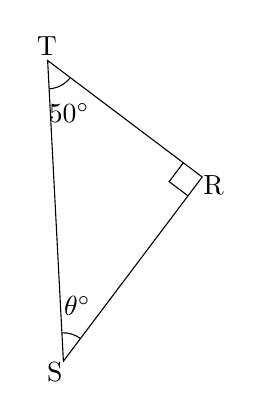
\begin{tikzpicture}[scale=1.2, baseline=(current bounding box.north)]

    \begin{scope}[rotate=273]
      \coordinate (A) at (0,0);
      \coordinate (B) at (3.1858082260731884,0);
      \coordinate (C) at (intersection cs: first line={(A)--($(A)+(50:4cm)$)}, second line={(B)--($(B)+(180-40:4cm)$)});
      \draw (A) -- (B) -- (C) -- cycle;

      % Mark angles with arcs
      \draw ($(A)!0.3cm!(B)$) arc [start angle=0, end angle=50, radius=0.3cm];
      \draw ($(B)!0.3cm!(C)$) arc [start angle=180-40, end angle=180, radius=0.3cm];
      % \draw ($(C)!0.3cm!(A)$) arc [start angle=180+50, end angle=360-40, radius=0.3cm];
      % rt angle mark at C
      % \tkzMarkRightAng0le(A,C,B); % uses \usepackage{tkz-euclide}
      \draw ($(C)!0.25cm!(A)$) -- ($(C)!0.25cm!(A)!0.25cm!90:(A)$) -- ($(C)!0.25cm!(B)$);
      %  The ($(C)!0.3cm!(A)!0.3cm!90:(A)$) syntax is used to specify a point that is 0.3cm away from the point ($(C)!0.3cm!(A)$) in a direction that is perpendicular to the line connecting points C and A. This is achieved by first specifying the point ($(C)!0.3cm!(A)$) and then rotating it by 90 degrees around point A using the !angle:anchor syntax.

      % Label angles
      \node at ($(A)!-0.15cm!(B)$) {T};
      \node at ($(B)!-0.15cm!(C)$) {S};
      \node at ($(C)!-0.15cm!(A)$) {R};

      % Mark angles in degrees
      \coordinate (midBC) at ($(B)!0.5!(C)$);
      \node at ($(A)!0.60cm!(midBC)$) {$50^\circ$};

      \coordinate (midAC) at ($(A)!0.5!(C)$);
      \node at ($(B)!0.60cm!(midAC)$) {$\theta^\circ$};

      % \coordinate (midAB) at ($(A)!0.5!(B)$);
      % \node at ($(C)!0.55cm!(midAB)$) {<<angleCValueDisplay>>$^\circ$};

    \end{scope}
  \end{tikzpicture}
\end{minipage}%
\hfill
\begin{minipage}{0.4\textwidth}
  \begin{align*}
    \angle \text{S} &= 90^\circ - \angle \text{\dotuline{~~~~~~~}} \\
    &= 90^\circ - \dotuline{~~~~~~~}^\circ  \\
    &= \dotuline{~~~~~~~}^\circ
  \end{align*}
\end{minipage}
\vspace{1cm}\begin{minipage}{0.55\textwidth}
  \refstepcounter{minipagecount}
  \noindent{(\theminipagecount)}\quad
  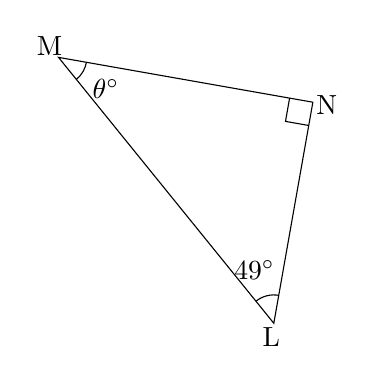
\begin{tikzpicture}[scale=1.2, baseline=(current bounding box.north)]

    \begin{scope}[rotate=309]
      \coordinate (A) at (0,0);
      \coordinate (B) at (3.6203307942976455,0);
      \coordinate (C) at (intersection cs: first line={(A)--($(A)+(41:4cm)$)}, second line={(B)--($(B)+(180-49:4cm)$)});
      \draw (A) -- (B) -- (C) -- cycle;

      % Mark angles with arcs
      \draw ($(A)!0.3cm!(B)$) arc [start angle=0, end angle=41, radius=0.3cm];
      \draw ($(B)!0.3cm!(C)$) arc [start angle=180-49, end angle=180, radius=0.3cm];
      % \draw ($(C)!0.3cm!(A)$) arc [start angle=180+41, end angle=360-49, radius=0.3cm];
      % rt angle mark at C
      % \tkzMarkRightAng0le(A,C,B); % uses \usepackage{tkz-euclide}
      \draw ($(C)!0.25cm!(A)$) -- ($(C)!0.25cm!(A)!0.25cm!90:(A)$) -- ($(C)!0.25cm!(B)$);
      %  The ($(C)!0.3cm!(A)!0.3cm!90:(A)$) syntax is used to specify a point that is 0.3cm away from the point ($(C)!0.3cm!(A)$) in a direction that is perpendicular to the line connecting points C and A. This is achieved by first specifying the point ($(C)!0.3cm!(A)$) and then rotating it by 90 degrees around point A using the !angle:anchor syntax.

      % Label angles
      \node at ($(A)!-0.15cm!(B)$) {M};
      \node at ($(B)!-0.15cm!(C)$) {L};
      \node at ($(C)!-0.15cm!(A)$) {N};

      % Mark angles in degrees
      \coordinate (midBC) at ($(B)!0.5!(C)$);
      \node at ($(A)!0.60cm!(midBC)$) {$\theta^\circ$};

      \coordinate (midAC) at ($(A)!0.5!(C)$);
      \node at ($(B)!0.60cm!(midAC)$) {$49^\circ$};

      % \coordinate (midAB) at ($(A)!0.5!(B)$);
      % \node at ($(C)!0.55cm!(midAB)$) {<<angleCValueDisplay>>$^\circ$};

    \end{scope}
  \end{tikzpicture}
\end{minipage}%
\hfill
\begin{minipage}{0.4\textwidth}
  \begin{align*}
    \angle \text{M} &= 90^\circ - \angle \text{\dotuline{~~~~~~~}} \\
    &= 90^\circ - \dotuline{~~~~~~~}^\circ  \\
    &= \dotuline{~~~~~~~}^\circ
  \end{align*}
\end{minipage}
\vspace{1cm}\begin{minipage}{0.55\textwidth}
  \refstepcounter{minipagecount}
  \noindent{(\theminipagecount)}\quad
  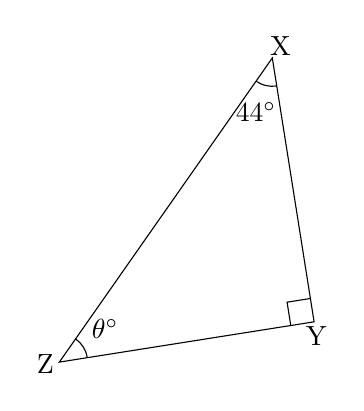
\begin{tikzpicture}[scale=1.2, baseline=(current bounding box.north)]

    \begin{scope}[rotate=235]
      \coordinate (A) at (0,0);
      \coordinate (B) at (3.9289540495496764,0);
      \coordinate (C) at (intersection cs: first line={(A)--($(A)+(44:4cm)$)}, second line={(B)--($(B)+(180-46:4cm)$)});
      \draw (A) -- (B) -- (C) -- cycle;

      % Mark angles with arcs
      \draw ($(A)!0.3cm!(B)$) arc [start angle=0, end angle=44, radius=0.3cm];
      \draw ($(B)!0.3cm!(C)$) arc [start angle=180-46, end angle=180, radius=0.3cm];
      % \draw ($(C)!0.3cm!(A)$) arc [start angle=180+44, end angle=360-46, radius=0.3cm];
      % rt angle mark at C
      % \tkzMarkRightAng0le(A,C,B); % uses \usepackage{tkz-euclide}
      \draw ($(C)!0.25cm!(A)$) -- ($(C)!0.25cm!(A)!0.25cm!90:(A)$) -- ($(C)!0.25cm!(B)$);
      %  The ($(C)!0.3cm!(A)!0.3cm!90:(A)$) syntax is used to specify a point that is 0.3cm away from the point ($(C)!0.3cm!(A)$) in a direction that is perpendicular to the line connecting points C and A. This is achieved by first specifying the point ($(C)!0.3cm!(A)$) and then rotating it by 90 degrees around point A using the !angle:anchor syntax.

      % Label angles
      \node at ($(A)!-0.15cm!(B)$) {X};
      \node at ($(B)!-0.15cm!(C)$) {Z};
      \node at ($(C)!-0.15cm!(A)$) {Y};

      % Mark angles in degrees
      \coordinate (midBC) at ($(B)!0.5!(C)$);
      \node at ($(A)!0.60cm!(midBC)$) {$44^\circ$};

      \coordinate (midAC) at ($(A)!0.5!(C)$);
      \node at ($(B)!0.60cm!(midAC)$) {$\theta^\circ$};

      % \coordinate (midAB) at ($(A)!0.5!(B)$);
      % \node at ($(C)!0.55cm!(midAB)$) {<<angleCValueDisplay>>$^\circ$};

    \end{scope}
  \end{tikzpicture}
\end{minipage}%
\hfill
\begin{minipage}{0.4\textwidth}
  \begin{align*}
    \angle \text{Z} &= 90^\circ - \angle \text{\dotuline{~~~~~~~}} \\
    &= 90^\circ - \dotuline{~~~~~~~}^\circ  \\
    &= \dotuline{~~~~~~~}^\circ
  \end{align*}
\end{minipage}
\vspace{1cm}\begin{minipage}{0.55\textwidth}
  \refstepcounter{minipagecount}
  \noindent{(\theminipagecount)}\quad
  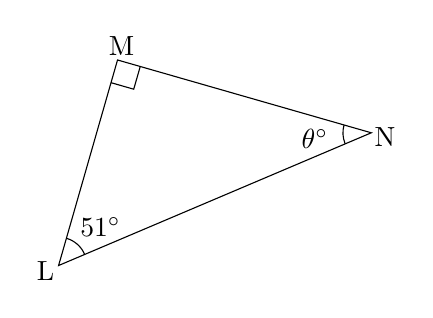
\begin{tikzpicture}[scale=1.2, baseline=(current bounding box.north)]

    \begin{scope}[rotate=23]
      \coordinate (A) at (0,0);
      \coordinate (B) at (3.594555090705758,0);
      \coordinate (C) at (intersection cs: first line={(A)--($(A)+(51:4cm)$)}, second line={(B)--($(B)+(180-39:4cm)$)});
      \draw (A) -- (B) -- (C) -- cycle;

      % Mark angles with arcs
      \draw ($(A)!0.3cm!(B)$) arc [start angle=0, end angle=51, radius=0.3cm];
      \draw ($(B)!0.3cm!(C)$) arc [start angle=180-39, end angle=180, radius=0.3cm];
      % \draw ($(C)!0.3cm!(A)$) arc [start angle=180+51, end angle=360-39, radius=0.3cm];
      % rt angle mark at C
      % \tkzMarkRightAng0le(A,C,B); % uses \usepackage{tkz-euclide}
      \draw ($(C)!0.25cm!(A)$) -- ($(C)!0.25cm!(A)!0.25cm!90:(A)$) -- ($(C)!0.25cm!(B)$);
      %  The ($(C)!0.3cm!(A)!0.3cm!90:(A)$) syntax is used to specify a point that is 0.3cm away from the point ($(C)!0.3cm!(A)$) in a direction that is perpendicular to the line connecting points C and A. This is achieved by first specifying the point ($(C)!0.3cm!(A)$) and then rotating it by 90 degrees around point A using the !angle:anchor syntax.

      % Label angles
      \node at ($(A)!-0.15cm!(B)$) {L};
      \node at ($(B)!-0.15cm!(C)$) {N};
      \node at ($(C)!-0.15cm!(A)$) {M};

      % Mark angles in degrees
      \coordinate (midBC) at ($(B)!0.5!(C)$);
      \node at ($(A)!0.60cm!(midBC)$) {$51^\circ$};

      \coordinate (midAC) at ($(A)!0.5!(C)$);
      \node at ($(B)!0.60cm!(midAC)$) {$\theta^\circ$};

      % \coordinate (midAB) at ($(A)!0.5!(B)$);
      % \node at ($(C)!0.55cm!(midAB)$) {<<angleCValueDisplay>>$^\circ$};

    \end{scope}
  \end{tikzpicture}
\end{minipage}%
\hfill
\begin{minipage}{0.4\textwidth}
  \begin{align*}
    \angle \text{N} &= 90^\circ - \angle \text{\dotuline{~~~~~~~}} \\
    &= 90^\circ - \dotuline{~~~~~~~}^\circ  \\
    &= \dotuline{~~~~~~~}^\circ
  \end{align*}
\end{minipage}
\vspace{1cm}\begin{minipage}{0.55\textwidth}
  \refstepcounter{minipagecount}
  \noindent{(\theminipagecount)}\quad
  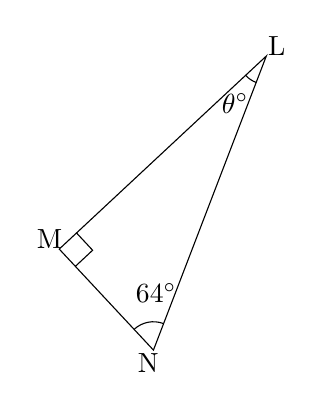
\begin{tikzpicture}[scale=1.2, baseline=(current bounding box.north)]

    \begin{scope}[rotate=69]
      \coordinate (A) at (0,0);
      \coordinate (B) at (3.3332590462389042,0);
      \coordinate (C) at (intersection cs: first line={(A)--($(A)+(64:4cm)$)}, second line={(B)--($(B)+(180-26:4cm)$)});
      \draw (A) -- (B) -- (C) -- cycle;

      % Mark angles with arcs
      \draw ($(A)!0.3cm!(B)$) arc [start angle=0, end angle=64, radius=0.3cm];
      \draw ($(B)!0.3cm!(C)$) arc [start angle=180-26, end angle=180, radius=0.3cm];
      % \draw ($(C)!0.3cm!(A)$) arc [start angle=180+64, end angle=360-26, radius=0.3cm];
      % rt angle mark at C
      % \tkzMarkRightAng0le(A,C,B); % uses \usepackage{tkz-euclide}
      \draw ($(C)!0.25cm!(A)$) -- ($(C)!0.25cm!(A)!0.25cm!90:(A)$) -- ($(C)!0.25cm!(B)$);
      %  The ($(C)!0.3cm!(A)!0.3cm!90:(A)$) syntax is used to specify a point that is 0.3cm away from the point ($(C)!0.3cm!(A)$) in a direction that is perpendicular to the line connecting points C and A. This is achieved by first specifying the point ($(C)!0.3cm!(A)$) and then rotating it by 90 degrees around point A using the !angle:anchor syntax.

      % Label angles
      \node at ($(A)!-0.15cm!(B)$) {N};
      \node at ($(B)!-0.15cm!(C)$) {L};
      \node at ($(C)!-0.15cm!(A)$) {M};

      % Mark angles in degrees
      \coordinate (midBC) at ($(B)!0.5!(C)$);
      \node at ($(A)!0.60cm!(midBC)$) {$64^\circ$};

      \coordinate (midAC) at ($(A)!0.5!(C)$);
      \node at ($(B)!0.60cm!(midAC)$) {$\theta^\circ$};

      % \coordinate (midAB) at ($(A)!0.5!(B)$);
      % \node at ($(C)!0.55cm!(midAB)$) {<<angleCValueDisplay>>$^\circ$};

    \end{scope}
  \end{tikzpicture}
\end{minipage}%
\hfill
\begin{minipage}{0.4\textwidth}
  \begin{align*}
    \angle \text{L} &= 90^\circ - \angle \text{\dotuline{~~~~~~~}} \\
    &= 90^\circ - \dotuline{~~~~~~~}^\circ  \\
    &= \dotuline{~~~~~~~}^\circ
  \end{align*}
\end{minipage}
\vspace{1cm}\begin{minipage}{0.55\textwidth}
  \refstepcounter{minipagecount}
  \noindent{(\theminipagecount)}\quad
  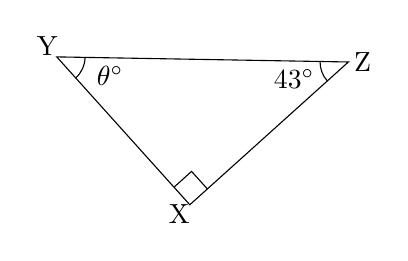
\begin{tikzpicture}[scale=1.2, baseline=(current bounding box.north)]

    \begin{scope}[rotate=179]
      \coordinate (A) at (0,0);
      \coordinate (B) at (3.086515549946404,0);
      \coordinate (C) at (intersection cs: first line={(A)--($(A)+(43:4cm)$)}, second line={(B)--($(B)+(180-47:4cm)$)});
      \draw (A) -- (B) -- (C) -- cycle;

      % Mark angles with arcs
      \draw ($(A)!0.3cm!(B)$) arc [start angle=0, end angle=43, radius=0.3cm];
      \draw ($(B)!0.3cm!(C)$) arc [start angle=180-47, end angle=180, radius=0.3cm];
      % \draw ($(C)!0.3cm!(A)$) arc [start angle=180+43, end angle=360-47, radius=0.3cm];
      % rt angle mark at C
      % \tkzMarkRightAng0le(A,C,B); % uses \usepackage{tkz-euclide}
      \draw ($(C)!0.25cm!(A)$) -- ($(C)!0.25cm!(A)!0.25cm!90:(A)$) -- ($(C)!0.25cm!(B)$);
      %  The ($(C)!0.3cm!(A)!0.3cm!90:(A)$) syntax is used to specify a point that is 0.3cm away from the point ($(C)!0.3cm!(A)$) in a direction that is perpendicular to the line connecting points C and A. This is achieved by first specifying the point ($(C)!0.3cm!(A)$) and then rotating it by 90 degrees around point A using the !angle:anchor syntax.

      % Label angles
      \node at ($(A)!-0.15cm!(B)$) {Z};
      \node at ($(B)!-0.15cm!(C)$) {Y};
      \node at ($(C)!-0.15cm!(A)$) {X};

      % Mark angles in degrees
      \coordinate (midBC) at ($(B)!0.5!(C)$);
      \node at ($(A)!0.60cm!(midBC)$) {$43^\circ$};

      \coordinate (midAC) at ($(A)!0.5!(C)$);
      \node at ($(B)!0.60cm!(midAC)$) {$\theta^\circ$};

      % \coordinate (midAB) at ($(A)!0.5!(B)$);
      % \node at ($(C)!0.55cm!(midAB)$) {<<angleCValueDisplay>>$^\circ$};

    \end{scope}
  \end{tikzpicture}
\end{minipage}%
\hfill
\begin{minipage}{0.4\textwidth}
  \begin{align*}
    \angle \text{Y} &= 90^\circ - \angle \text{\dotuline{~~~~~~~}} \\
    &= 90^\circ - \dotuline{~~~~~~~}^\circ  \\
    &= \dotuline{~~~~~~~}^\circ
  \end{align*}
\end{minipage}
\vspace{1cm}\begin{minipage}{0.55\textwidth}
  \refstepcounter{minipagecount}
  \noindent{(\theminipagecount)}\quad
  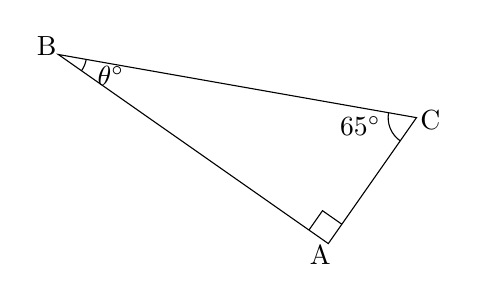
\begin{tikzpicture}[scale=1.2, baseline=(current bounding box.north)]

    \begin{scope}[rotate=170]
      \coordinate (A) at (0,0);
      \coordinate (B) at (3.848616513291856,0);
      \coordinate (C) at (intersection cs: first line={(A)--($(A)+(65:4cm)$)}, second line={(B)--($(B)+(180-25:4cm)$)});
      \draw (A) -- (B) -- (C) -- cycle;

      % Mark angles with arcs
      \draw ($(A)!0.3cm!(B)$) arc [start angle=0, end angle=65, radius=0.3cm];
      \draw ($(B)!0.3cm!(C)$) arc [start angle=180-25, end angle=180, radius=0.3cm];
      % \draw ($(C)!0.3cm!(A)$) arc [start angle=180+65, end angle=360-25, radius=0.3cm];
      % rt angle mark at C
      % \tkzMarkRightAng0le(A,C,B); % uses \usepackage{tkz-euclide}
      \draw ($(C)!0.25cm!(A)$) -- ($(C)!0.25cm!(A)!0.25cm!90:(A)$) -- ($(C)!0.25cm!(B)$);
      %  The ($(C)!0.3cm!(A)!0.3cm!90:(A)$) syntax is used to specify a point that is 0.3cm away from the point ($(C)!0.3cm!(A)$) in a direction that is perpendicular to the line connecting points C and A. This is achieved by first specifying the point ($(C)!0.3cm!(A)$) and then rotating it by 90 degrees around point A using the !angle:anchor syntax.

      % Label angles
      \node at ($(A)!-0.15cm!(B)$) {C};
      \node at ($(B)!-0.15cm!(C)$) {B};
      \node at ($(C)!-0.15cm!(A)$) {A};

      % Mark angles in degrees
      \coordinate (midBC) at ($(B)!0.5!(C)$);
      \node at ($(A)!0.60cm!(midBC)$) {$65^\circ$};

      \coordinate (midAC) at ($(A)!0.5!(C)$);
      \node at ($(B)!0.60cm!(midAC)$) {$\theta^\circ$};

      % \coordinate (midAB) at ($(A)!0.5!(B)$);
      % \node at ($(C)!0.55cm!(midAB)$) {<<angleCValueDisplay>>$^\circ$};

    \end{scope}
  \end{tikzpicture}
\end{minipage}%
\hfill
\begin{minipage}{0.4\textwidth}
  \begin{align*}
    \angle \text{B} &= 90^\circ - \angle \text{\dotuline{~~~~~~~}} \\
    &= 90^\circ - \dotuline{~~~~~~~}^\circ  \\
    &= \dotuline{~~~~~~~}^\circ
  \end{align*}
\end{minipage}
\vspace{1cm}\begin{minipage}{0.55\textwidth}
  \refstepcounter{minipagecount}
  \noindent{(\theminipagecount)}\quad
  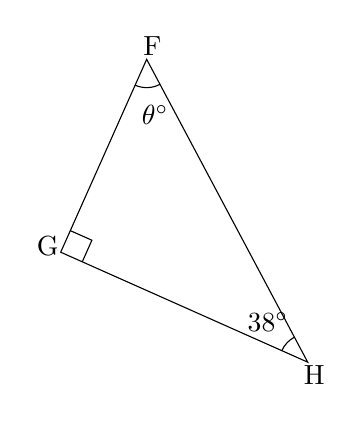
\begin{tikzpicture}[scale=1.2, baseline=(current bounding box.north)]

    \begin{scope}[rotate=118]
      \coordinate (A) at (0,0);
      \coordinate (B) at (3.6300624247175337,0);
      \coordinate (C) at (intersection cs: first line={(A)--($(A)+(38:4cm)$)}, second line={(B)--($(B)+(180-52:4cm)$)});
      \draw (A) -- (B) -- (C) -- cycle;

      % Mark angles with arcs
      \draw ($(A)!0.3cm!(B)$) arc [start angle=0, end angle=38, radius=0.3cm];
      \draw ($(B)!0.3cm!(C)$) arc [start angle=180-52, end angle=180, radius=0.3cm];
      % \draw ($(C)!0.3cm!(A)$) arc [start angle=180+38, end angle=360-52, radius=0.3cm];
      % rt angle mark at C
      % \tkzMarkRightAng0le(A,C,B); % uses \usepackage{tkz-euclide}
      \draw ($(C)!0.25cm!(A)$) -- ($(C)!0.25cm!(A)!0.25cm!90:(A)$) -- ($(C)!0.25cm!(B)$);
      %  The ($(C)!0.3cm!(A)!0.3cm!90:(A)$) syntax is used to specify a point that is 0.3cm away from the point ($(C)!0.3cm!(A)$) in a direction that is perpendicular to the line connecting points C and A. This is achieved by first specifying the point ($(C)!0.3cm!(A)$) and then rotating it by 90 degrees around point A using the !angle:anchor syntax.

      % Label angles
      \node at ($(A)!-0.15cm!(B)$) {H};
      \node at ($(B)!-0.15cm!(C)$) {F};
      \node at ($(C)!-0.15cm!(A)$) {G};

      % Mark angles in degrees
      \coordinate (midBC) at ($(B)!0.5!(C)$);
      \node at ($(A)!0.60cm!(midBC)$) {$38^\circ$};

      \coordinate (midAC) at ($(A)!0.5!(C)$);
      \node at ($(B)!0.60cm!(midAC)$) {$\theta^\circ$};

      % \coordinate (midAB) at ($(A)!0.5!(B)$);
      % \node at ($(C)!0.55cm!(midAB)$) {<<angleCValueDisplay>>$^\circ$};

    \end{scope}
  \end{tikzpicture}
\end{minipage}%
\hfill
\begin{minipage}{0.4\textwidth}
  \begin{align*}
    \angle \text{F} &= 90^\circ - \angle \text{\dotuline{~~~~~~~}} \\
    &= 90^\circ - \dotuline{~~~~~~~}^\circ  \\
    &= \dotuline{~~~~~~~}^\circ
  \end{align*}
\end{minipage}
\vspace{1cm}\begin{minipage}{0.55\textwidth}
  \refstepcounter{minipagecount}
  \noindent{(\theminipagecount)}\quad
  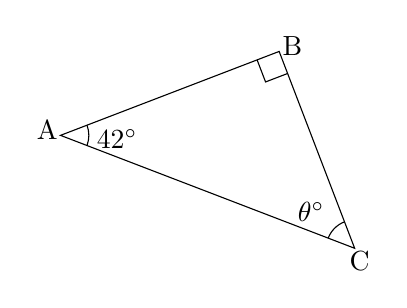
\begin{tikzpicture}[scale=1.2, baseline=(current bounding box.north)]

    \begin{scope}[rotate=339]
      \coordinate (A) at (0,0);
      \coordinate (B) at (3.3341107507606704,0);
      \coordinate (C) at (intersection cs: first line={(A)--($(A)+(42:4cm)$)}, second line={(B)--($(B)+(180-48:4cm)$)});
      \draw (A) -- (B) -- (C) -- cycle;

      % Mark angles with arcs
      \draw ($(A)!0.3cm!(B)$) arc [start angle=0, end angle=42, radius=0.3cm];
      \draw ($(B)!0.3cm!(C)$) arc [start angle=180-48, end angle=180, radius=0.3cm];
      % \draw ($(C)!0.3cm!(A)$) arc [start angle=180+42, end angle=360-48, radius=0.3cm];
      % rt angle mark at C
      % \tkzMarkRightAng0le(A,C,B); % uses \usepackage{tkz-euclide}
      \draw ($(C)!0.25cm!(A)$) -- ($(C)!0.25cm!(A)!0.25cm!90:(A)$) -- ($(C)!0.25cm!(B)$);
      %  The ($(C)!0.3cm!(A)!0.3cm!90:(A)$) syntax is used to specify a point that is 0.3cm away from the point ($(C)!0.3cm!(A)$) in a direction that is perpendicular to the line connecting points C and A. This is achieved by first specifying the point ($(C)!0.3cm!(A)$) and then rotating it by 90 degrees around point A using the !angle:anchor syntax.

      % Label angles
      \node at ($(A)!-0.15cm!(B)$) {A};
      \node at ($(B)!-0.15cm!(C)$) {C};
      \node at ($(C)!-0.15cm!(A)$) {B};

      % Mark angles in degrees
      \coordinate (midBC) at ($(B)!0.5!(C)$);
      \node at ($(A)!0.60cm!(midBC)$) {$42^\circ$};

      \coordinate (midAC) at ($(A)!0.5!(C)$);
      \node at ($(B)!0.60cm!(midAC)$) {$\theta^\circ$};

      % \coordinate (midAB) at ($(A)!0.5!(B)$);
      % \node at ($(C)!0.55cm!(midAB)$) {<<angleCValueDisplay>>$^\circ$};

    \end{scope}
  \end{tikzpicture}
\end{minipage}%
\hfill
\begin{minipage}{0.4\textwidth}
  \begin{align*}
    \angle \text{C} &= 90^\circ - \angle \text{\dotuline{~~~~~~~}} \\
    &= 90^\circ - \dotuline{~~~~~~~}^\circ  \\
    &= \dotuline{~~~~~~~}^\circ
  \end{align*}
\end{minipage}
\vspace{1cm}\begin{minipage}{0.55\textwidth}
  \refstepcounter{minipagecount}
  \noindent{(\theminipagecount)}\quad
  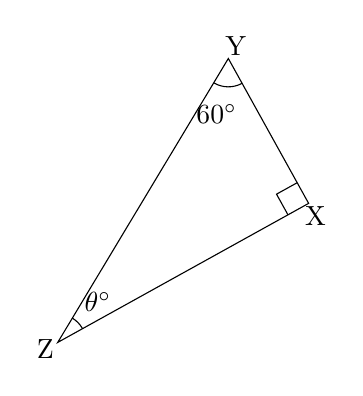
\begin{tikzpicture}[scale=1.2, baseline=(current bounding box.north)]

    \begin{scope}[rotate=239]
      \coordinate (A) at (0,0);
      \coordinate (B) at (3.5049433024657377,0);
      \coordinate (C) at (intersection cs: first line={(A)--($(A)+(60:4cm)$)}, second line={(B)--($(B)+(180-30:4cm)$)});
      \draw (A) -- (B) -- (C) -- cycle;

      % Mark angles with arcs
      \draw ($(A)!0.3cm!(B)$) arc [start angle=0, end angle=60, radius=0.3cm];
      \draw ($(B)!0.3cm!(C)$) arc [start angle=180-30, end angle=180, radius=0.3cm];
      % \draw ($(C)!0.3cm!(A)$) arc [start angle=180+60, end angle=360-30, radius=0.3cm];
      % rt angle mark at C
      % \tkzMarkRightAng0le(A,C,B); % uses \usepackage{tkz-euclide}
      \draw ($(C)!0.25cm!(A)$) -- ($(C)!0.25cm!(A)!0.25cm!90:(A)$) -- ($(C)!0.25cm!(B)$);
      %  The ($(C)!0.3cm!(A)!0.3cm!90:(A)$) syntax is used to specify a point that is 0.3cm away from the point ($(C)!0.3cm!(A)$) in a direction that is perpendicular to the line connecting points C and A. This is achieved by first specifying the point ($(C)!0.3cm!(A)$) and then rotating it by 90 degrees around point A using the !angle:anchor syntax.

      % Label angles
      \node at ($(A)!-0.15cm!(B)$) {Y};
      \node at ($(B)!-0.15cm!(C)$) {Z};
      \node at ($(C)!-0.15cm!(A)$) {X};

      % Mark angles in degrees
      \coordinate (midBC) at ($(B)!0.5!(C)$);
      \node at ($(A)!0.60cm!(midBC)$) {$60^\circ$};

      \coordinate (midAC) at ($(A)!0.5!(C)$);
      \node at ($(B)!0.60cm!(midAC)$) {$\theta^\circ$};

      % \coordinate (midAB) at ($(A)!0.5!(B)$);
      % \node at ($(C)!0.55cm!(midAB)$) {<<angleCValueDisplay>>$^\circ$};

    \end{scope}
  \end{tikzpicture}
\end{minipage}%
\hfill
\begin{minipage}{0.4\textwidth}
  \begin{align*}
    \angle \text{Z} &= 90^\circ - \angle \text{\dotuline{~~~~~~~}} \\
    &= 90^\circ - \dotuline{~~~~~~~}^\circ  \\
    &= \dotuline{~~~~~~~}^\circ
  \end{align*}
\end{minipage}
\vspace{1cm}\begin{minipage}{0.55\textwidth}
  \refstepcounter{minipagecount}
  \noindent{(\theminipagecount)}\quad
  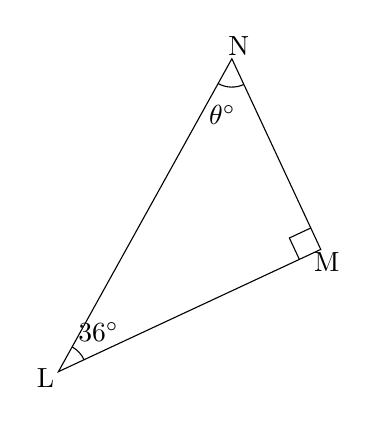
\begin{tikzpicture}[scale=1.2, baseline=(current bounding box.north)]

    \begin{scope}[rotate=241]
      \coordinate (A) at (0,0);
      \coordinate (B) at (3.786310973646671,0);
      \coordinate (C) at (intersection cs: first line={(A)--($(A)+(54:4cm)$)}, second line={(B)--($(B)+(180-36:4cm)$)});
      \draw (A) -- (B) -- (C) -- cycle;

      % Mark angles with arcs
      \draw ($(A)!0.3cm!(B)$) arc [start angle=0, end angle=54, radius=0.3cm];
      \draw ($(B)!0.3cm!(C)$) arc [start angle=180-36, end angle=180, radius=0.3cm];
      % \draw ($(C)!0.3cm!(A)$) arc [start angle=180+54, end angle=360-36, radius=0.3cm];
      % rt angle mark at C
      % \tkzMarkRightAng0le(A,C,B); % uses \usepackage{tkz-euclide}
      \draw ($(C)!0.25cm!(A)$) -- ($(C)!0.25cm!(A)!0.25cm!90:(A)$) -- ($(C)!0.25cm!(B)$);
      %  The ($(C)!0.3cm!(A)!0.3cm!90:(A)$) syntax is used to specify a point that is 0.3cm away from the point ($(C)!0.3cm!(A)$) in a direction that is perpendicular to the line connecting points C and A. This is achieved by first specifying the point ($(C)!0.3cm!(A)$) and then rotating it by 90 degrees around point A using the !angle:anchor syntax.

      % Label angles
      \node at ($(A)!-0.15cm!(B)$) {N};
      \node at ($(B)!-0.15cm!(C)$) {L};
      \node at ($(C)!-0.15cm!(A)$) {M};

      % Mark angles in degrees
      \coordinate (midBC) at ($(B)!0.5!(C)$);
      \node at ($(A)!0.60cm!(midBC)$) {$\theta^\circ$};

      \coordinate (midAC) at ($(A)!0.5!(C)$);
      \node at ($(B)!0.60cm!(midAC)$) {$36^\circ$};

      % \coordinate (midAB) at ($(A)!0.5!(B)$);
      % \node at ($(C)!0.55cm!(midAB)$) {<<angleCValueDisplay>>$^\circ$};

    \end{scope}
  \end{tikzpicture}
\end{minipage}%
\hfill
\begin{minipage}{0.4\textwidth}
  \begin{align*}
    \angle \text{N} &= 90^\circ - \angle \text{\dotuline{~~~~~~~}} \\
    &= 90^\circ - \dotuline{~~~~~~~}^\circ  \\
    &= \dotuline{~~~~~~~}^\circ
  \end{align*}
\end{minipage}
\vspace{1cm}\begin{minipage}{0.55\textwidth}
  \refstepcounter{minipagecount}
  \noindent{(\theminipagecount)}\quad
  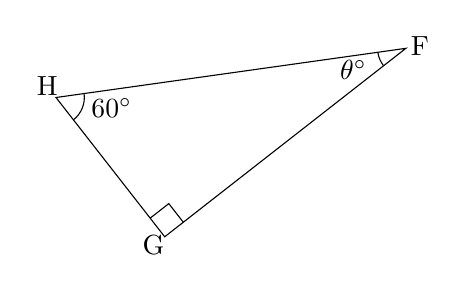
\begin{tikzpicture}[scale=1.2, baseline=(current bounding box.north)]

    \begin{scope}[rotate=188]
      \coordinate (A) at (0,0);
      \coordinate (B) at (3.7392307906783744,0);
      \coordinate (C) at (intersection cs: first line={(A)--($(A)+(30:4cm)$)}, second line={(B)--($(B)+(180-60:4cm)$)});
      \draw (A) -- (B) -- (C) -- cycle;

      % Mark angles with arcs
      \draw ($(A)!0.3cm!(B)$) arc [start angle=0, end angle=30, radius=0.3cm];
      \draw ($(B)!0.3cm!(C)$) arc [start angle=180-60, end angle=180, radius=0.3cm];
      % \draw ($(C)!0.3cm!(A)$) arc [start angle=180+30, end angle=360-60, radius=0.3cm];
      % rt angle mark at C
      % \tkzMarkRightAng0le(A,C,B); % uses \usepackage{tkz-euclide}
      \draw ($(C)!0.25cm!(A)$) -- ($(C)!0.25cm!(A)!0.25cm!90:(A)$) -- ($(C)!0.25cm!(B)$);
      %  The ($(C)!0.3cm!(A)!0.3cm!90:(A)$) syntax is used to specify a point that is 0.3cm away from the point ($(C)!0.3cm!(A)$) in a direction that is perpendicular to the line connecting points C and A. This is achieved by first specifying the point ($(C)!0.3cm!(A)$) and then rotating it by 90 degrees around point A using the !angle:anchor syntax.

      % Label angles
      \node at ($(A)!-0.15cm!(B)$) {F};
      \node at ($(B)!-0.15cm!(C)$) {H};
      \node at ($(C)!-0.15cm!(A)$) {G};

      % Mark angles in degrees
      \coordinate (midBC) at ($(B)!0.5!(C)$);
      \node at ($(A)!0.60cm!(midBC)$) {$\theta^\circ$};

      \coordinate (midAC) at ($(A)!0.5!(C)$);
      \node at ($(B)!0.60cm!(midAC)$) {$60^\circ$};

      % \coordinate (midAB) at ($(A)!0.5!(B)$);
      % \node at ($(C)!0.55cm!(midAB)$) {<<angleCValueDisplay>>$^\circ$};

    \end{scope}
  \end{tikzpicture}
\end{minipage}%
\hfill
\begin{minipage}{0.4\textwidth}
  \begin{align*}
    \angle \text{F} &= 90^\circ - \angle \text{\dotuline{~~~~~~~}} \\
    &= 90^\circ - \dotuline{~~~~~~~}^\circ  \\
    &= \dotuline{~~~~~~~}^\circ
  \end{align*}
\end{minipage}
\vspace{1cm}\begin{minipage}{0.55\textwidth}
  \refstepcounter{minipagecount}
  \noindent{(\theminipagecount)}\quad
  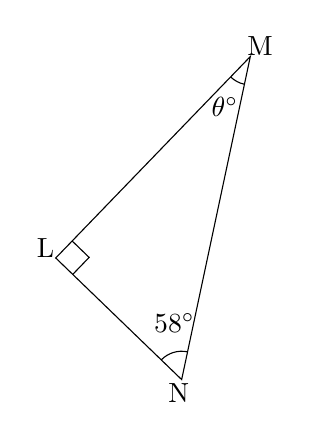
\begin{tikzpicture}[scale=1.2, baseline=(current bounding box.north)]

    \begin{scope}[rotate=78]
      \coordinate (A) at (0,0);
      \coordinate (B) at (3.4947481031691887,0);
      \coordinate (C) at (intersection cs: first line={(A)--($(A)+(58:4cm)$)}, second line={(B)--($(B)+(180-32:4cm)$)});
      \draw (A) -- (B) -- (C) -- cycle;

      % Mark angles with arcs
      \draw ($(A)!0.3cm!(B)$) arc [start angle=0, end angle=58, radius=0.3cm];
      \draw ($(B)!0.3cm!(C)$) arc [start angle=180-32, end angle=180, radius=0.3cm];
      % \draw ($(C)!0.3cm!(A)$) arc [start angle=180+58, end angle=360-32, radius=0.3cm];
      % rt angle mark at C
      % \tkzMarkRightAng0le(A,C,B); % uses \usepackage{tkz-euclide}
      \draw ($(C)!0.25cm!(A)$) -- ($(C)!0.25cm!(A)!0.25cm!90:(A)$) -- ($(C)!0.25cm!(B)$);
      %  The ($(C)!0.3cm!(A)!0.3cm!90:(A)$) syntax is used to specify a point that is 0.3cm away from the point ($(C)!0.3cm!(A)$) in a direction that is perpendicular to the line connecting points C and A. This is achieved by first specifying the point ($(C)!0.3cm!(A)$) and then rotating it by 90 degrees around point A using the !angle:anchor syntax.

      % Label angles
      \node at ($(A)!-0.15cm!(B)$) {N};
      \node at ($(B)!-0.15cm!(C)$) {M};
      \node at ($(C)!-0.15cm!(A)$) {L};

      % Mark angles in degrees
      \coordinate (midBC) at ($(B)!0.5!(C)$);
      \node at ($(A)!0.60cm!(midBC)$) {$58^\circ$};

      \coordinate (midAC) at ($(A)!0.5!(C)$);
      \node at ($(B)!0.60cm!(midAC)$) {$\theta^\circ$};

      % \coordinate (midAB) at ($(A)!0.5!(B)$);
      % \node at ($(C)!0.55cm!(midAB)$) {<<angleCValueDisplay>>$^\circ$};

    \end{scope}
  \end{tikzpicture}
\end{minipage}%
\hfill
\begin{minipage}{0.4\textwidth}
  \begin{align*}
    \angle \text{M} &= 90^\circ - \angle \text{\dotuline{~~~~~~~}} \\
    &= 90^\circ - \dotuline{~~~~~~~}^\circ  \\
    &= \dotuline{~~~~~~~}^\circ
  \end{align*}
\end{minipage}
\vspace{1cm}\begin{minipage}{0.55\textwidth}
  \refstepcounter{minipagecount}
  \noindent{(\theminipagecount)}\quad
  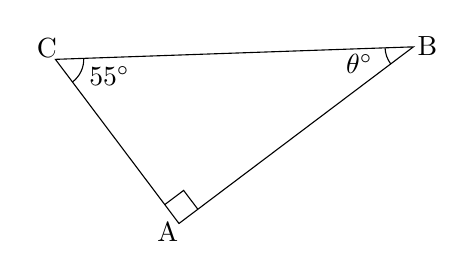
\begin{tikzpicture}[scale=1.2, baseline=(current bounding box.north)]

    \begin{scope}[rotate=182]
      \coordinate (A) at (0,0);
      \coordinate (B) at (3.790094151453448,0);
      \coordinate (C) at (intersection cs: first line={(A)--($(A)+(35:4cm)$)}, second line={(B)--($(B)+(180-55:4cm)$)});
      \draw (A) -- (B) -- (C) -- cycle;

      % Mark angles with arcs
      \draw ($(A)!0.3cm!(B)$) arc [start angle=0, end angle=35, radius=0.3cm];
      \draw ($(B)!0.3cm!(C)$) arc [start angle=180-55, end angle=180, radius=0.3cm];
      % \draw ($(C)!0.3cm!(A)$) arc [start angle=180+35, end angle=360-55, radius=0.3cm];
      % rt angle mark at C
      % \tkzMarkRightAng0le(A,C,B); % uses \usepackage{tkz-euclide}
      \draw ($(C)!0.25cm!(A)$) -- ($(C)!0.25cm!(A)!0.25cm!90:(A)$) -- ($(C)!0.25cm!(B)$);
      %  The ($(C)!0.3cm!(A)!0.3cm!90:(A)$) syntax is used to specify a point that is 0.3cm away from the point ($(C)!0.3cm!(A)$) in a direction that is perpendicular to the line connecting points C and A. This is achieved by first specifying the point ($(C)!0.3cm!(A)$) and then rotating it by 90 degrees around point A using the !angle:anchor syntax.

      % Label angles
      \node at ($(A)!-0.15cm!(B)$) {B};
      \node at ($(B)!-0.15cm!(C)$) {C};
      \node at ($(C)!-0.15cm!(A)$) {A};

      % Mark angles in degrees
      \coordinate (midBC) at ($(B)!0.5!(C)$);
      \node at ($(A)!0.60cm!(midBC)$) {$\theta^\circ$};

      \coordinate (midAC) at ($(A)!0.5!(C)$);
      \node at ($(B)!0.60cm!(midAC)$) {$55^\circ$};

      % \coordinate (midAB) at ($(A)!0.5!(B)$);
      % \node at ($(C)!0.55cm!(midAB)$) {<<angleCValueDisplay>>$^\circ$};

    \end{scope}
  \end{tikzpicture}
\end{minipage}%
\hfill
\begin{minipage}{0.4\textwidth}
  \begin{align*}
    \angle \text{B} &= 90^\circ - \angle \text{\dotuline{~~~~~~~}} \\
    &= 90^\circ - \dotuline{~~~~~~~}^\circ  \\
    &= \dotuline{~~~~~~~}^\circ
  \end{align*}
\end{minipage}
\vspace{1cm}\begin{minipage}{0.55\textwidth}
  \refstepcounter{minipagecount}
  \noindent{(\theminipagecount)}\quad
  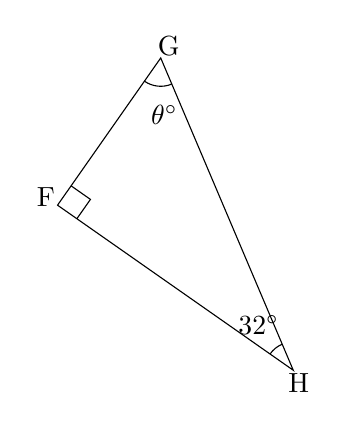
\begin{tikzpicture}[scale=1.2, baseline=(current bounding box.north)]

    \begin{scope}[rotate=113]
      \coordinate (A) at (0,0);
      \coordinate (B) at (3.5900932949595425,0);
      \coordinate (C) at (intersection cs: first line={(A)--($(A)+(32:4cm)$)}, second line={(B)--($(B)+(180-58:4cm)$)});
      \draw (A) -- (B) -- (C) -- cycle;

      % Mark angles with arcs
      \draw ($(A)!0.3cm!(B)$) arc [start angle=0, end angle=32, radius=0.3cm];
      \draw ($(B)!0.3cm!(C)$) arc [start angle=180-58, end angle=180, radius=0.3cm];
      % \draw ($(C)!0.3cm!(A)$) arc [start angle=180+32, end angle=360-58, radius=0.3cm];
      % rt angle mark at C
      % \tkzMarkRightAng0le(A,C,B); % uses \usepackage{tkz-euclide}
      \draw ($(C)!0.25cm!(A)$) -- ($(C)!0.25cm!(A)!0.25cm!90:(A)$) -- ($(C)!0.25cm!(B)$);
      %  The ($(C)!0.3cm!(A)!0.3cm!90:(A)$) syntax is used to specify a point that is 0.3cm away from the point ($(C)!0.3cm!(A)$) in a direction that is perpendicular to the line connecting points C and A. This is achieved by first specifying the point ($(C)!0.3cm!(A)$) and then rotating it by 90 degrees around point A using the !angle:anchor syntax.

      % Label angles
      \node at ($(A)!-0.15cm!(B)$) {H};
      \node at ($(B)!-0.15cm!(C)$) {G};
      \node at ($(C)!-0.15cm!(A)$) {F};

      % Mark angles in degrees
      \coordinate (midBC) at ($(B)!0.5!(C)$);
      \node at ($(A)!0.60cm!(midBC)$) {$32^\circ$};

      \coordinate (midAC) at ($(A)!0.5!(C)$);
      \node at ($(B)!0.60cm!(midAC)$) {$\theta^\circ$};

      % \coordinate (midAB) at ($(A)!0.5!(B)$);
      % \node at ($(C)!0.55cm!(midAB)$) {<<angleCValueDisplay>>$^\circ$};

    \end{scope}
  \end{tikzpicture}
\end{minipage}%
\hfill
\begin{minipage}{0.4\textwidth}
  \begin{align*}
    \angle \text{G} &= 90^\circ - \angle \text{\dotuline{~~~~~~~}} \\
    &= 90^\circ - \dotuline{~~~~~~~}^\circ  \\
    &= \dotuline{~~~~~~~}^\circ
  \end{align*}
\end{minipage}
\vspace{1cm}\begin{minipage}{0.55\textwidth}
  \refstepcounter{minipagecount}
  \noindent{(\theminipagecount)}\quad
  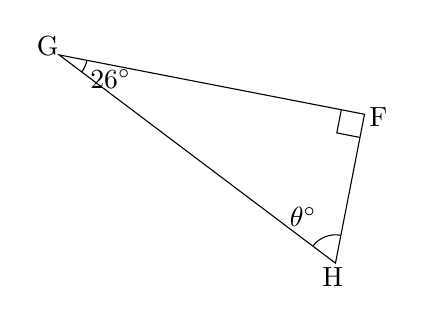
\begin{tikzpicture}[scale=1.2, baseline=(current bounding box.north)]

    \begin{scope}[rotate=323]
      \coordinate (A) at (0,0);
      \coordinate (B) at (3.662090820686853,0);
      \coordinate (C) at (intersection cs: first line={(A)--($(A)+(26:4cm)$)}, second line={(B)--($(B)+(180-64:4cm)$)});
      \draw (A) -- (B) -- (C) -- cycle;

      % Mark angles with arcs
      \draw ($(A)!0.3cm!(B)$) arc [start angle=0, end angle=26, radius=0.3cm];
      \draw ($(B)!0.3cm!(C)$) arc [start angle=180-64, end angle=180, radius=0.3cm];
      % \draw ($(C)!0.3cm!(A)$) arc [start angle=180+26, end angle=360-64, radius=0.3cm];
      % rt angle mark at C
      % \tkzMarkRightAng0le(A,C,B); % uses \usepackage{tkz-euclide}
      \draw ($(C)!0.25cm!(A)$) -- ($(C)!0.25cm!(A)!0.25cm!90:(A)$) -- ($(C)!0.25cm!(B)$);
      %  The ($(C)!0.3cm!(A)!0.3cm!90:(A)$) syntax is used to specify a point that is 0.3cm away from the point ($(C)!0.3cm!(A)$) in a direction that is perpendicular to the line connecting points C and A. This is achieved by first specifying the point ($(C)!0.3cm!(A)$) and then rotating it by 90 degrees around point A using the !angle:anchor syntax.

      % Label angles
      \node at ($(A)!-0.15cm!(B)$) {G};
      \node at ($(B)!-0.15cm!(C)$) {H};
      \node at ($(C)!-0.15cm!(A)$) {F};

      % Mark angles in degrees
      \coordinate (midBC) at ($(B)!0.5!(C)$);
      \node at ($(A)!0.60cm!(midBC)$) {$26^\circ$};

      \coordinate (midAC) at ($(A)!0.5!(C)$);
      \node at ($(B)!0.60cm!(midAC)$) {$\theta^\circ$};

      % \coordinate (midAB) at ($(A)!0.5!(B)$);
      % \node at ($(C)!0.55cm!(midAB)$) {<<angleCValueDisplay>>$^\circ$};

    \end{scope}
  \end{tikzpicture}
\end{minipage}%
\hfill
\begin{minipage}{0.4\textwidth}
  \begin{align*}
    \angle \text{H} &= 90^\circ - \angle \text{\dotuline{~~~~~~~}} \\
    &= 90^\circ - \dotuline{~~~~~~~}^\circ  \\
    &= \dotuline{~~~~~~~}^\circ
  \end{align*}
\end{minipage}
\vspace{1cm}\begin{minipage}{0.55\textwidth}
  \refstepcounter{minipagecount}
  \noindent{(\theminipagecount)}\quad
  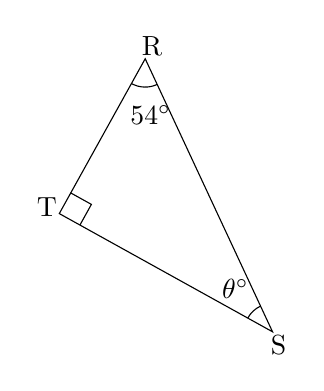
\begin{tikzpicture}[scale=1.2, baseline=(current bounding box.north)]

    \begin{scope}[rotate=115]
      \coordinate (A) at (0,0);
      \coordinate (B) at (3.188040593058351,0);
      \coordinate (C) at (intersection cs: first line={(A)--($(A)+(36:4cm)$)}, second line={(B)--($(B)+(180-54:4cm)$)});
      \draw (A) -- (B) -- (C) -- cycle;

      % Mark angles with arcs
      \draw ($(A)!0.3cm!(B)$) arc [start angle=0, end angle=36, radius=0.3cm];
      \draw ($(B)!0.3cm!(C)$) arc [start angle=180-54, end angle=180, radius=0.3cm];
      % \draw ($(C)!0.3cm!(A)$) arc [start angle=180+36, end angle=360-54, radius=0.3cm];
      % rt angle mark at C
      % \tkzMarkRightAng0le(A,C,B); % uses \usepackage{tkz-euclide}
      \draw ($(C)!0.25cm!(A)$) -- ($(C)!0.25cm!(A)!0.25cm!90:(A)$) -- ($(C)!0.25cm!(B)$);
      %  The ($(C)!0.3cm!(A)!0.3cm!90:(A)$) syntax is used to specify a point that is 0.3cm away from the point ($(C)!0.3cm!(A)$) in a direction that is perpendicular to the line connecting points C and A. This is achieved by first specifying the point ($(C)!0.3cm!(A)$) and then rotating it by 90 degrees around point A using the !angle:anchor syntax.

      % Label angles
      \node at ($(A)!-0.15cm!(B)$) {S};
      \node at ($(B)!-0.15cm!(C)$) {R};
      \node at ($(C)!-0.15cm!(A)$) {T};

      % Mark angles in degrees
      \coordinate (midBC) at ($(B)!0.5!(C)$);
      \node at ($(A)!0.60cm!(midBC)$) {$\theta^\circ$};

      \coordinate (midAC) at ($(A)!0.5!(C)$);
      \node at ($(B)!0.60cm!(midAC)$) {$54^\circ$};

      % \coordinate (midAB) at ($(A)!0.5!(B)$);
      % \node at ($(C)!0.55cm!(midAB)$) {<<angleCValueDisplay>>$^\circ$};

    \end{scope}
  \end{tikzpicture}
\end{minipage}%
\hfill
\begin{minipage}{0.4\textwidth}
  \begin{align*}
    \angle \text{S} &= 90^\circ - \angle \text{\dotuline{~~~~~~~}} \\
    &= 90^\circ - \dotuline{~~~~~~~}^\circ  \\
    &= \dotuline{~~~~~~~}^\circ
  \end{align*}
\end{minipage}
\vspace{1cm}\begin{minipage}{0.55\textwidth}
  \refstepcounter{minipagecount}
  \noindent{(\theminipagecount)}\quad
  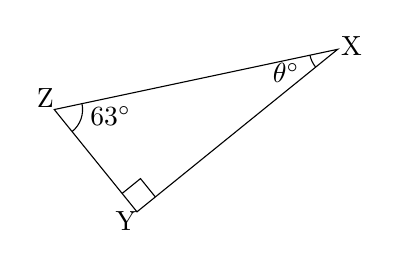
\begin{tikzpicture}[scale=1.2, baseline=(current bounding box.north)]

    \begin{scope}[rotate=192]
      \coordinate (A) at (0,0);
      \coordinate (B) at (3.066113222980716,0);
      \coordinate (C) at (intersection cs: first line={(A)--($(A)+(27:4cm)$)}, second line={(B)--($(B)+(180-63:4cm)$)});
      \draw (A) -- (B) -- (C) -- cycle;

      % Mark angles with arcs
      \draw ($(A)!0.3cm!(B)$) arc [start angle=0, end angle=27, radius=0.3cm];
      \draw ($(B)!0.3cm!(C)$) arc [start angle=180-63, end angle=180, radius=0.3cm];
      % \draw ($(C)!0.3cm!(A)$) arc [start angle=180+27, end angle=360-63, radius=0.3cm];
      % rt angle mark at C
      % \tkzMarkRightAng0le(A,C,B); % uses \usepackage{tkz-euclide}
      \draw ($(C)!0.25cm!(A)$) -- ($(C)!0.25cm!(A)!0.25cm!90:(A)$) -- ($(C)!0.25cm!(B)$);
      %  The ($(C)!0.3cm!(A)!0.3cm!90:(A)$) syntax is used to specify a point that is 0.3cm away from the point ($(C)!0.3cm!(A)$) in a direction that is perpendicular to the line connecting points C and A. This is achieved by first specifying the point ($(C)!0.3cm!(A)$) and then rotating it by 90 degrees around point A using the !angle:anchor syntax.

      % Label angles
      \node at ($(A)!-0.15cm!(B)$) {X};
      \node at ($(B)!-0.15cm!(C)$) {Z};
      \node at ($(C)!-0.15cm!(A)$) {Y};

      % Mark angles in degrees
      \coordinate (midBC) at ($(B)!0.5!(C)$);
      \node at ($(A)!0.60cm!(midBC)$) {$\theta^\circ$};

      \coordinate (midAC) at ($(A)!0.5!(C)$);
      \node at ($(B)!0.60cm!(midAC)$) {$63^\circ$};

      % \coordinate (midAB) at ($(A)!0.5!(B)$);
      % \node at ($(C)!0.55cm!(midAB)$) {<<angleCValueDisplay>>$^\circ$};

    \end{scope}
  \end{tikzpicture}
\end{minipage}%
\hfill
\begin{minipage}{0.4\textwidth}
  \begin{align*}
    \angle \text{X} &= 90^\circ - \angle \text{\dotuline{~~~~~~~}} \\
    &= 90^\circ - \dotuline{~~~~~~~}^\circ  \\
    &= \dotuline{~~~~~~~}^\circ
  \end{align*}
\end{minipage}
\vspace{1cm}\begin{minipage}{0.55\textwidth}
  \refstepcounter{minipagecount}
  \noindent{(\theminipagecount)}\quad
  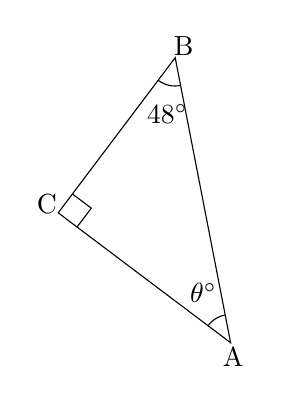
\begin{tikzpicture}[scale=1.2, baseline=(current bounding box.north)]

    \begin{scope}[rotate=101]
      \coordinate (A) at (0,0);
      \coordinate (B) at (3.0729273170728795,0);
      \coordinate (C) at (intersection cs: first line={(A)--($(A)+(42:4cm)$)}, second line={(B)--($(B)+(180-48:4cm)$)});
      \draw (A) -- (B) -- (C) -- cycle;

      % Mark angles with arcs
      \draw ($(A)!0.3cm!(B)$) arc [start angle=0, end angle=42, radius=0.3cm];
      \draw ($(B)!0.3cm!(C)$) arc [start angle=180-48, end angle=180, radius=0.3cm];
      % \draw ($(C)!0.3cm!(A)$) arc [start angle=180+42, end angle=360-48, radius=0.3cm];
      % rt angle mark at C
      % \tkzMarkRightAng0le(A,C,B); % uses \usepackage{tkz-euclide}
      \draw ($(C)!0.25cm!(A)$) -- ($(C)!0.25cm!(A)!0.25cm!90:(A)$) -- ($(C)!0.25cm!(B)$);
      %  The ($(C)!0.3cm!(A)!0.3cm!90:(A)$) syntax is used to specify a point that is 0.3cm away from the point ($(C)!0.3cm!(A)$) in a direction that is perpendicular to the line connecting points C and A. This is achieved by first specifying the point ($(C)!0.3cm!(A)$) and then rotating it by 90 degrees around point A using the !angle:anchor syntax.

      % Label angles
      \node at ($(A)!-0.15cm!(B)$) {A};
      \node at ($(B)!-0.15cm!(C)$) {B};
      \node at ($(C)!-0.15cm!(A)$) {C};

      % Mark angles in degrees
      \coordinate (midBC) at ($(B)!0.5!(C)$);
      \node at ($(A)!0.60cm!(midBC)$) {$\theta^\circ$};

      \coordinate (midAC) at ($(A)!0.5!(C)$);
      \node at ($(B)!0.60cm!(midAC)$) {$48^\circ$};

      % \coordinate (midAB) at ($(A)!0.5!(B)$);
      % \node at ($(C)!0.55cm!(midAB)$) {<<angleCValueDisplay>>$^\circ$};

    \end{scope}
  \end{tikzpicture}
\end{minipage}%
\hfill
\begin{minipage}{0.4\textwidth}
  \begin{align*}
    \angle \text{A} &= 90^\circ - \angle \text{\dotuline{~~~~~~~}} \\
    &= 90^\circ - \dotuline{~~~~~~~}^\circ  \\
    &= \dotuline{~~~~~~~}^\circ
  \end{align*}
\end{minipage}
\vspace{1cm}

\end{document}
